% *** Authors should verify (and, if needed, correct) their LaTeX system  ***
% *** with the testflow diagnostic prior to trusting their LaTeX platform ***
% *** with production work. IEEE's font choices can trigger bugs that do  ***
% *** not appear when using other class files.                            ***
% The testflow support page is at:
% http://www.michaelshell.org/tex/testflow/


%%*************************************************************************
%% Legal Notice:
%% This code is offered as-is without any warranty either expressed or
%% implied; without even the implied warranty of MERCHANTABILITY or
%% FITNESS FOR A PARTICULAR PURPOSE!
%% User assumes all risk.
%% In no event shall IEEE or any contributor to this code be liable for
%% any damages or losses, including, but not limited to, incidental,
%% consequential, or any other damages, resulting from the use or misuse
%% of any information contained here.
%%
%% All comments are the opinions of their respective authors and are not
%% necessarily endorsed by the IEEE.
%%
%% This work is distributed under the LaTeX Project Public License (LPPL)
%% ( http://www.latex-project.org/ ) version 1.3, and may be freely used,
%% distributed and modified. A copy of the LPPL, version 1.3, is included
%% in the base LaTeX documentation of all distributions of LaTeX released
%% 2003/12/01 or later.
%% Retain all contribution notices and credits.
%% ** Modified files should be clearly indicated as such, including  **
%% ** renaming them and changing author support contact information. **
%%
%% File list of work: IEEEtran.cls, New_IEEEtran_how-to.pdf, bare_jrnl_new_sample4.tex,
%%*************************************************************************
\PassOptionsToPackage{unicode}{hyperref}
\PassOptionsToPackage{hyphens}{url}
\PassOptionsToPackage{dvipsnames,svgnames,x11names}{xcolor}
% Note that the a4paper option is mainly intended so that authors in
% countries using A4 can easily print to A4 and see how their papers will
% look in print - the typesetting of the document will not typically be
% affected with changes in paper size (but the bottom and side margins will).
% Use the testflow package mentioned above to verify correct handling of
% both paper sizes by the user's LaTeX system.
%
% Also note that the "draftcls" or "draftclsnofoot", not "draft", option
% should be used if it is desired that the figures are to be displayed in
% draft mode.
%
\documentclass[
  journal,
]{IEEEtran}%
% If IEEEtran.cls has not been installed into the LaTeX system files,
% manually specify the path to it like:
% \documentclass[journal]{../sty/IEEEtran}
\usepackage[cmex10]{amsmath}
\usepackage{amssymb}
\usepackage{iftex}
\ifPDFTeX
  \usepackage[T1]{fontenc}
  \usepackage[utf8]{inputenc}
  \usepackage{textcomp} % provide euro and other symbols
\else % if luatex or xetex
  \usepackage{unicode-math} % this also loads fontspec
  \defaultfontfeatures{Scale=MatchLowercase}
  \defaultfontfeatures[\rmfamily]{Ligatures=TeX,Scale=1}
\fi
%\usepackage{lmodern}
\ifPDFTeX\else
\fi
% Use upquote if available, for straight quotes in verbatim environments
\IfFileExists{upquote.sty}{\usepackage{upquote}}{}
\IfFileExists{microtype.sty}{% use microtype if available
  \usepackage[]{microtype}
  \UseMicrotypeSet[protrusion]{basicmath} % disable protrusion for tt fonts
}{}
\makeatletter
\parindent    1.0em
\ifCLASSOPTIONcompsoc
  \parindent    1.5em
\fi
\makeatother
\usepackage{xcolor}
\setlength{\emergencystretch}{3em} % prevent overfull lines

\setcounter{secnumdepth}{5}
% Make \paragraph and \subparagraph free-standing
\ifx\paragraph\undefined\else
  \let\oldparagraph\paragraph
  \renewcommand{\paragraph}[1]{\oldparagraph{#1}\mbox{}}
\fi
\ifx\subparagraph\undefined\else
  \let\oldsubparagraph\subparagraph
  \renewcommand{\subparagraph}[1]{\oldsubparagraph{#1}\mbox{}}
\fi

\usepackage{color}
\usepackage{fancyvrb}
\newcommand{\VerbBar}{|}
\newcommand{\VERB}{\Verb[commandchars=\\\{\}]}
\DefineVerbatimEnvironment{Highlighting}{Verbatim}{commandchars=\\\{\}}
% Add ',fontsize=\small' for more characters per line
\usepackage{framed}
\definecolor{shadecolor}{RGB}{241,243,245}
\newenvironment{Shaded}{\begin{snugshade}}{\end{snugshade}}
\newcommand{\AlertTok}[1]{\textcolor[rgb]{0.68,0.00,0.00}{#1}}
\newcommand{\AnnotationTok}[1]{\textcolor[rgb]{0.37,0.37,0.37}{#1}}
\newcommand{\AttributeTok}[1]{\textcolor[rgb]{0.40,0.45,0.13}{#1}}
\newcommand{\BaseNTok}[1]{\textcolor[rgb]{0.68,0.00,0.00}{#1}}
\newcommand{\BuiltInTok}[1]{\textcolor[rgb]{0.00,0.23,0.31}{#1}}
\newcommand{\CharTok}[1]{\textcolor[rgb]{0.13,0.47,0.30}{#1}}
\newcommand{\CommentTok}[1]{\textcolor[rgb]{0.37,0.37,0.37}{#1}}
\newcommand{\CommentVarTok}[1]{\textcolor[rgb]{0.37,0.37,0.37}{\textit{#1}}}
\newcommand{\ConstantTok}[1]{\textcolor[rgb]{0.56,0.35,0.01}{#1}}
\newcommand{\ControlFlowTok}[1]{\textcolor[rgb]{0.00,0.23,0.31}{\textbf{#1}}}
\newcommand{\DataTypeTok}[1]{\textcolor[rgb]{0.68,0.00,0.00}{#1}}
\newcommand{\DecValTok}[1]{\textcolor[rgb]{0.68,0.00,0.00}{#1}}
\newcommand{\DocumentationTok}[1]{\textcolor[rgb]{0.37,0.37,0.37}{\textit{#1}}}
\newcommand{\ErrorTok}[1]{\textcolor[rgb]{0.68,0.00,0.00}{#1}}
\newcommand{\ExtensionTok}[1]{\textcolor[rgb]{0.00,0.23,0.31}{#1}}
\newcommand{\FloatTok}[1]{\textcolor[rgb]{0.68,0.00,0.00}{#1}}
\newcommand{\FunctionTok}[1]{\textcolor[rgb]{0.28,0.35,0.67}{#1}}
\newcommand{\ImportTok}[1]{\textcolor[rgb]{0.00,0.46,0.62}{#1}}
\newcommand{\InformationTok}[1]{\textcolor[rgb]{0.37,0.37,0.37}{#1}}
\newcommand{\KeywordTok}[1]{\textcolor[rgb]{0.00,0.23,0.31}{\textbf{#1}}}
\newcommand{\NormalTok}[1]{\textcolor[rgb]{0.00,0.23,0.31}{#1}}
\newcommand{\OperatorTok}[1]{\textcolor[rgb]{0.37,0.37,0.37}{#1}}
\newcommand{\OtherTok}[1]{\textcolor[rgb]{0.00,0.23,0.31}{#1}}
\newcommand{\PreprocessorTok}[1]{\textcolor[rgb]{0.68,0.00,0.00}{#1}}
\newcommand{\RegionMarkerTok}[1]{\textcolor[rgb]{0.00,0.23,0.31}{#1}}
\newcommand{\SpecialCharTok}[1]{\textcolor[rgb]{0.37,0.37,0.37}{#1}}
\newcommand{\SpecialStringTok}[1]{\textcolor[rgb]{0.13,0.47,0.30}{#1}}
\newcommand{\StringTok}[1]{\textcolor[rgb]{0.13,0.47,0.30}{#1}}
\newcommand{\VariableTok}[1]{\textcolor[rgb]{0.07,0.07,0.07}{#1}}
\newcommand{\VerbatimStringTok}[1]{\textcolor[rgb]{0.13,0.47,0.30}{#1}}
\newcommand{\WarningTok}[1]{\textcolor[rgb]{0.37,0.37,0.37}{\textit{#1}}}

\providecommand{\tightlist}{%
  \setlength{\itemsep}{0pt}\setlength{\parskip}{0pt}}\usepackage{longtable,booktabs,array}
\usepackage{calc} % for calculating minipage widths
% Correct order of tables after \paragraph or \subparagraph
\usepackage{etoolbox}
\makeatletter
\patchcmd\longtable{\par}{\if@noskipsec\mbox{}\fi\par}{}{}
\makeatother
% Allow footnotes in longtable head/foot
\IfFileExists{footnotehyper.sty}{\usepackage{footnotehyper}}{\usepackage{footnote}}
\makesavenoteenv{longtable}
\usepackage{graphicx}
\makeatletter
\def\maxwidth{\ifdim\Gin@nat@width>\linewidth\linewidth\else\Gin@nat@width\fi}
\def\maxheight{\ifdim\Gin@nat@height>\textheight\textheight\else\Gin@nat@height\fi}
\makeatother
% Scale images if necessary, so that they will not overflow the page
% margins by default, and it is still possible to overwrite the defaults
% using explicit options in \includegraphics[width, height, ...]{}
\setkeys{Gin}{width=\maxwidth,height=\maxheight,keepaspectratio}
% Set default figure placement to htbp
\makeatletter
\def\fps@figure{htbp}
\makeatother
% definitions for citeproc citations
\NewDocumentCommand\citeproctext{}{}
\NewDocumentCommand\citeproc{mm}{%
  \begingroup\def\citeproctext{#2}\cite{#1}\endgroup}
\makeatletter
 % allow citations to break across lines
 \let\@cite@ofmt\@firstofone
 % avoid brackets around text for \cite:
 \def\@biblabel#1{}
 \def\@cite#1#2{{#1\if@tempswa , #2\fi}}
\makeatother
\newlength{\cslhangindent}
\setlength{\cslhangindent}{1.5em}
\newlength{\csllabelwidth}
\setlength{\csllabelwidth}{3em}
\newenvironment{CSLReferences}[2] % #1 hanging-indent, #2 entry-spacing
 {\begin{list}{}{%
  \setlength{\itemindent}{0pt}
  \setlength{\leftmargin}{0pt}
  \setlength{\parsep}{0pt}
  % turn on hanging indent if param 1 is 1
  \ifodd #1
   \setlength{\leftmargin}{\cslhangindent}
   \setlength{\itemindent}{-1\cslhangindent}
  \fi
  % set entry spacing
  \setlength{\itemsep}{#2\baselineskip}}}
 {\end{list}}
\usepackage{calc}
\newcommand{\CSLBlock}[1]{\hfill\break\parbox[t]{\linewidth}{\strut\ignorespaces#1\strut}}
\newcommand{\CSLLeftMargin}[1]{\parbox[t]{\csllabelwidth}{\strut#1\strut}}
\newcommand{\CSLRightInline}[1]{\parbox[t]{\linewidth - \csllabelwidth}{\strut#1\strut}}
\newcommand{\CSLIndent}[1]{\hspace{\cslhangindent}#1}

\usepackage{booktabs}
\usepackage{longtable}
\usepackage{array}
\usepackage{multirow}
\usepackage{wrapfig}
\usepackage{float}
\usepackage{colortbl}
\usepackage{pdflscape}
\usepackage{tabu}
\usepackage{threeparttable}
\usepackage{threeparttablex}
\usepackage[normalem]{ulem}
\usepackage{makecell}
\usepackage{xcolor}
\usepackage{physics}
\usepackage[version=3]{mhchem}
\usepackage{orcidlink}
\usepackage{float}
\floatplacement{table}{htb}
\usepackage[english]{babel}
\usepackage{bm,bbm}
\usepackage{mathrsfs}
\usepackage{siunitx}
\usepackage{graphicx}
\usepackage{url}
\usepackage[T1]{fontenc}
\usepackage{polski}
\usepackage{booktabs}
\usepackage{color}
\usepackage{xcolor}
\usepackage{amsmath}
\usepackage{multirow}
\usepackage{subcaption}
\captionsetup[subfigure]{labelformat=parens, justification=centering}
\usepackage{placeins}
\makeatletter
\@ifpackageloaded{caption}{}{\usepackage{caption}}
\AtBeginDocument{%
\ifdefined\contentsname
  \renewcommand*\contentsname{Table of contents}
\else
  \newcommand\contentsname{Table of contents}
\fi
\ifdefined\listfigurename
  \renewcommand*\listfigurename{List of Figures}
\else
  \newcommand\listfigurename{List of Figures}
\fi
\ifdefined\listtablename
  \renewcommand*\listtablename{List of Tables}
\else
  \newcommand\listtablename{List of Tables}
\fi
\ifdefined\figurename
  \renewcommand*\figurename{Fig.}
\else
  \newcommand\figurename{Fig.}
\fi
\ifdefined\tablename
  \renewcommand*\tablename{Table}
\else
  \newcommand\tablename{Table}
\fi
}
\@ifpackageloaded{float}{}{\usepackage{float}}
\floatstyle{ruled}
\@ifundefined{c@chapter}{\newfloat{codelisting}{h}{lop}}{\newfloat{codelisting}{h}{lop}[chapter]}
\floatname{codelisting}{Listing}
\newcommand*\listoflistings{\listof{codelisting}{List of Listings}}
\makeatother
\makeatletter
\makeatother
\makeatletter
\@ifpackageloaded{caption}{}{\usepackage{caption}}
\@ifpackageloaded{subcaption}{}{\usepackage{subcaption}}
\makeatother
\usepackage[skip=2pt,font=footnotesize]{caption}
%\captionsetup{format=myformat}
\makeatletter
%\setlength{\cslhangindent}{0pt plus .5pt}
\providecommand{\bibfont}{\footnotesize}
\let\CSLReferences@rig=\CSLReferences
\renewcommand{\CSLReferences}[2]{
\bibfont\settowidth\csllabelwidth{[999]}
\CSLReferences@rig{#1}{#2}
\vskip 0.3\baselineskip plus 0.1\baselineskip minus 0.1\baselineskip%
}
\makeatother
\ifLuaTeX
  \usepackage{selnolig}  % disable illegal ligatures
\fi
\IfFileExists{bookmark.sty}{\usepackage{bookmark}}{\usepackage{hyperref}}
\IfFileExists{xurl.sty}{\usepackage{xurl}}{} % add URL line breaks if available
\urlstyle{same} % disable monospaced font for URLs
\hypersetup{
  pdftitle={A Sample Article Using quarto-ieee for IEEE Journal and Transactions},
  pdfauthor={David Folio; John Doe},
  pdfkeywords={IEEE, IEEEtran, journal, Quarto, Pandoc, template},
  colorlinks=true,
  linkcolor={blue},
  filecolor={Maroon},
  citecolor={Blue},
  urlcolor={Blue},
  pdfcreator={LaTeX via pandoc}}

% *** Do not adjust lengths that control margins, column widths, etc. ***
% *** Do not use packages that alter fonts (such as pslatex).         ***
% There should be no need to do such things with IEEEtran.cls V1.6 and later.
% (Unless specifically asked to do so by the journal or conference you plan
% to submit to, of course. )


% correct bad hyphenation here
\hyphenation{op-tical net-works semi-conduc-tor}

%
% paper title
% can use linebreaks \\ within to get better formatting as desired
% Do not put math or special symbols in the title.
% paper title
% can use linebreaks \\ within to get better formatting as desired
% Do not put math or special symbols in the title.
\title{A Sample Article Using \texttt{quarto-ieee} for IEEE Journal and
Transactions}

\author{
\thanks{The \texttt{quarto-ieee} template is freely available under the
MIT license on github: \url{https://github.com/dfolio/quarto-ieee}.}
David Folio\orcidlink{0000-0001-9430-6091},~\IEEEmembership{Member,
IEEE}
and~John Doe%
\thanks{David Folio is with Laboratoire Prisme, INSA Centre Val de
Loire, Bourges, 18800 France%
  Corresponding author: david.folio@insa-cvl.fr
}
\thanks{Unknown affiliation}
%by-author.affiliations
\thanks{John Doe is with Anonymous University%
}
%by-author.affiliations
}
\begin{document}

% The paper headers
\markboth{Journal XXX, Month Year}{D. Folio: A Sample Article Using
quarto-ieee}

% use for special paper notices

% make the title area
\maketitle

% As a general rule, do not put math, special symbols or citations
% in the abstract or keywords.
\begin{abstract}
This document describes the most common article elements and how to use
the \texttt{quarto-ieee} class with Pandoc/Quarto-Markdown to produce
files that are suitable for submission to IEEE journals.
\texttt{quarto-ieee} can produce conference, journal, and technical note
(correspondence) papers with a suitable choice of class options. It
intends to generate PDF and HTML outputs that closely mimick what IEEE
would generate.
\end{abstract}
% Note that keywords are not normally used for peerreview papers.
\begin{IEEEkeywords}
IEEE, IEEEtran, journal, Quarto, Pandoc, template
\end{IEEEkeywords}

% For peer review papers, you can put extra information on the cover
% page as needed:
% \ifCLASSOPTIONpeerreview
% \begin{center} \bfseries EDICS Category: 3-BBND \end{center}
% \fi
%
% For peerreview papers, this IEEEtran command inserts a page break and
% creates the second title. It will be ignored for other modes.
% \IEEEpeerreviewmaketitle


\section{How to Use Cache in Quarto}\label{sec-intro}

\subsection{Global Cache}\label{global-cache}

First, we need to activate the cache globally for the entire document.
This means that all chunks that are executed will be cached and will not
be executed again unless there is a change in the code or dependencies.

\begin{Shaded}
\begin{Highlighting}[]
\InformationTok{\textasciigrave{}\textasciigrave{}\textasciigrave{}\{r setup, include=FALSE\}}
\InformationTok{knitr::opts\_chunk$set(echo = FALSE, }
\InformationTok{                              cache=TRUE)}
\InformationTok{\textasciigrave{}\textasciigrave{}\textasciigrave{}}
\end{Highlighting}
\end{Shaded}

\subsection{Simple Plot Example with Global
Cache}\label{simple-plot-example-with-global-cache}

This chunk uses the global cache. After the first execution, the cached
result will be used, so the plot won't be regenerated unless the code or
data changes.

\begin{Shaded}
\begin{Highlighting}[]
\FunctionTok{set.seed}\NormalTok{(}\DecValTok{123}\NormalTok{)}
\NormalTok{data }\OtherTok{\textless{}{-}} \FunctionTok{rnorm}\NormalTok{(}\DecValTok{1000}\NormalTok{)}

\FunctionTok{plot}\NormalTok{(}\FunctionTok{density}\NormalTok{(data), }\AttributeTok{main =} \StringTok{"plot"}\NormalTok{)}
\end{Highlighting}
\end{Shaded}

\subsection{Cache in a Specific Chunk}\label{cache-in-a-specific-chunk}

This chunk caches the summary table calculation. The table will only be
recalculated if the code or the data changes.

\subsection{Using if (!file.exists(\ldots)) to Save
Data}\label{using-if-file.exists-to-save-data}

This chunk uses the if (!file.exists(\ldots)) condition to avoid
recalculating the data if the file already exists. If the file exists,
it loads the saved data; otherwise, it runs the computation and saves
the results to the file. This approach is useful for collaboration,
where you can share the file and avoid recomputation on other machines.

\begin{Shaded}
\begin{Highlighting}[]
\CommentTok{\# This code will be displayed in the document}

\CommentTok{\# Check if the data file exists and save the results}

\ControlFlowTok{if}\NormalTok{ (}\SpecialCharTok{!}\FunctionTok{file.exists}\NormalTok{(}\StringTok{"saved\_data.Rdata"}\NormalTok{)) \{}

\NormalTok{  computed\_data }\OtherTok{\textless{}{-}} \FunctionTok{rnorm}\NormalTok{(}\DecValTok{1000}\NormalTok{)}
  \FunctionTok{save}\NormalTok{(computed\_data, }\AttributeTok{file =} \StringTok{"./Data/example\_data.Rdata"}\NormalTok{)}
\NormalTok{\} }\ControlFlowTok{else}\NormalTok{ \{}
  
  \CommentTok{\# Load the saved data}
  \FunctionTok{load}\NormalTok{(}\StringTok{"./Data/example\_data.Rdata"}\NormalTok{)}
\NormalTok{\}}

\CommentTok{\# }
\FunctionTok{head}\NormalTok{(computed\_data)}
\end{Highlighting}
\end{Shaded}

\subsection{eval: false}\label{eval-false}

\begin{Shaded}
\begin{Highlighting}[]
\CommentTok{\# This chunk will display the code}
\CommentTok{\# but will not execute it}
\FunctionTok{set.seed}\NormalTok{(}\DecValTok{123}\NormalTok{)}
\NormalTok{data }\OtherTok{\textless{}{-}} \FunctionTok{rnorm}\NormalTok{(}\DecValTok{1000}\NormalTok{)}
\FunctionTok{plot}\NormalTok{(}\FunctionTok{density}\NormalTok{(data), }\AttributeTok{main =} \StringTok{"plot"}\NormalTok{)}
\end{Highlighting}
\end{Shaded}

\section{Other examples: Plot and
table}\label{other-examples-plot-and-table}

In a famous paper, \citeproc{ref-BC64}{{[}1{]}} introduced a family of
transformations \dots

\begin{figure}[H]

\centering{

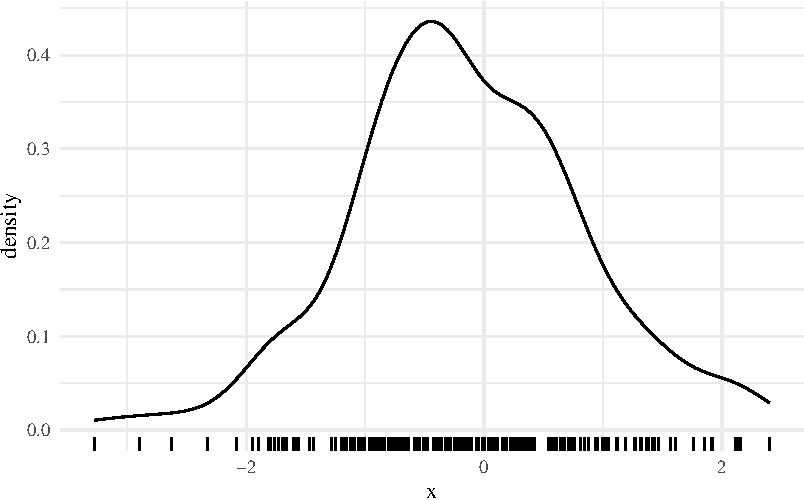
\includegraphics{ieee-template_files/figure-pdf/fig-density0-1.pdf}

}

\caption{\label{fig-density0}Simulated data from a N(0,1) distribution.}

\end{figure}%

Fig.~\ref{fig-density0} shows a kernel density estimate of simulated
data from a N(0,1) distribution. The sample variance is given by
\begin{equation}\phantomsection\label{eq-s2}{
  s^2 = \frac{1}{n-1} \sum_{i=1}^n (x_i-\bar{x})^2 = 0.98.
}\end{equation} Note that \ref{eq-s2} is an unbiased estimate of the
variance, but it is not the maximum likelihood estimate
\citeproc{ref-Rice2007}{{[}2, p. 269{]}}.

In table \ref{tab:time} we have \ldots{}

\section{Markdown basics}\label{sec-Markdown}

The reader can easily find many documentations on how to write using the
(Pandoc/Quarto) Markdown syntax. The \texttt{quarto-ieee} template
relies mainly on the Markdown markup supported by Quarto
\citeproc{ref-quarto-markdown}{{[}3{]}}, which is build based on Pandoc
\citeproc{ref-MacFarlane_Pandoc}{{[}4{]}},
\citeproc{ref-Allaire_Quarto_2022}{{[}5{]}}. Below are some basic
examples of usage of the Markdown markup (to save space, it is better to
consult the original Quarto document \texttt{template.qmd}).

\subsection{Figures}\label{figures}

An image with nonempty alt text will be rendered as a figure with a
caption with Pandoc and Quarto. Quarto includes a different features to
simplify the use of figures and subfigures. Here, it is recommended to
use div block with \texttt{\#fig-} label to embed your Figures.

\begin{figure}

\centering{

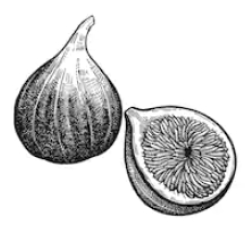
\includegraphics[width=0.3\textwidth,height=\textheight]{fig1.png}

}

\caption{\label{fig-1}An example of figure.}

\end{figure}%

\begin{figure}

\begin{minipage}{0.50\linewidth}

\centering{

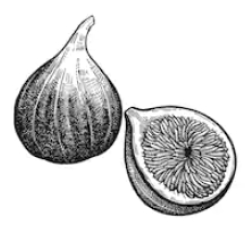
\includegraphics{fig1.png}

}

\subcaption{\label{fig-2a}}

\end{minipage}%
%
\begin{minipage}{0.50\linewidth}

\centering{

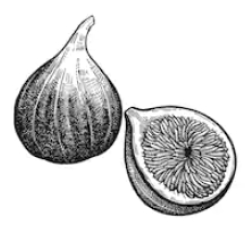
\includegraphics{fig1.png}

}

\subcaption{\label{fig-2b}}

\end{minipage}%

\caption{\label{fig-2}An example with sub-figure.}

\end{figure}%

The figures is cross-referenced as Fig.~\ref{fig-2} and even the
sub-figures as Fig.~\ref{fig-2b}.

\subsubsection{Tables}\label{sec-tables}

Similarly, many kind of tables may be used with Pandoc and Quarto. The
latter also includes different features to simplify the table output. To
make tables cross-referenceable use a label with a \texttt{\#tbl-}
prefix.\\
However, it is recommended to avoid using the commonly used single
Markdown table known as a `pipe table'. In fact, Pandoc Markdown uses
the {\LaTeX} \texttt{longtable} package, which does not support the
two-column mode, which is required for most \texttt{IEEEtran} journals.
\texttt{quarto-ieee} uses a hack to temporarily switch to one-column
mode. However, this hack may break the page layout. To overcome this
issue, a basic way is to use code cells (as for Table~\ref{tbl-other}).
Quarto is a multi-language and it uses \texttt{Knitr} to execute
\texttt{R} code and can execute Python code blocks within Markdown.

\begin{table}

\caption{\label{tbl-panel}Main Caption}

\begin{minipage}{0.50\linewidth}

\subcaption{\label{tbl-first}First Table}

\centering{

\begin{tabular}{lll}
\toprule
Col1 & Col2 & Col3\\
\midrule
A & B & C\\
E & F & G\\
A & G & G\\
\bottomrule
\end{tabular}

}

\end{minipage}%
%
\begin{minipage}{0.50\linewidth}

\subcaption{\label{tbl-second}Second Table}

\centering{

\begin{tabular}{lll}
\toprule
Col1 & Col2 & Col3\\
\midrule
A & B & C\\
E & F & G\\
A & G & G\\
\bottomrule
\end{tabular}

}

\end{minipage}%

\end{table}%

The Tables are cross-referenced as Table~\ref{tbl-panel} for details,
especially Table~\ref{tbl-second}. There is also Table~\ref{tbl-other}.

\subsection{Bibliography}\label{bibliography}

IEEE journal should normally use IEEEtran\footnote{IEEEtran BibTeX style
  support page is:
  \url{http://www.michaelshell.org/tex/ieeetran/bibtex/}}
\textsc{Bib}{\TeX} style. Nevertheless, Pandoc and Quarto do support
\textsc{Bib}{\TeX} with natbib or biblatex. However, neither is
officially recommended for normal IEEE use. For this reason,
\texttt{quarto-ieee} uses \texttt{citeproc} with the \texttt{ieee} CSL
style sheet.

\section{Conclusions}\label{conclusions}

The conclusion goes here.

\section*{Acknowledgment}\label{acknowledgment}
\addcontentsline{toc}{section}{Acknowledgment}

\appendix[An Appendix]{}

Use \texttt{{[}{]}\{.appendix\ options="An\ Appendix"\}} markup if you
have a single appendix. \texttt{IEEEtran} state that to do not use
\texttt{\textbackslash{}section\{\}} anymore after
\texttt{\textbackslash{}appendix}.

\section*{References}\label{references}
\addcontentsline{toc}{section}{References}

\phantomsection\label{refs}
\begin{CSLReferences}{0}{0}
\bibitem[\citeproctext]{ref-BC64}
\CSLLeftMargin{{[}1{]} }%
\CSLRightInline{G. E. P. Box and D. R. Cox, {``An analysis of
transformations,''} \emph{Journal of the Royal Statistical Society,
Series B}, vol. 26, no. 2, pp. 211--252, 1964. }

\bibitem[\citeproctext]{ref-Rice2007}
\CSLLeftMargin{{[}2{]} }%
\CSLRightInline{J. A. Rice, \emph{Mathematical statistics and data
analysis}, 3rd edition. Duxbury, 2007. }

\bibitem[\citeproctext]{ref-quarto-markdown}
\CSLLeftMargin{{[}3{]} }%
\CSLRightInline{{``Quarto - {Markdown Basics}.''} {[}Online{]}.
Available: \url{https://quarto.org/docs/authoring/markdown-basics}.
{[}Accessed: 25-Oct-2023{]}}

\bibitem[\citeproctext]{ref-MacFarlane_Pandoc}
\CSLLeftMargin{{[}4{]} }%
\CSLRightInline{J. MacFarlane, A. Krewinkel, and J. Rosenthal,
{``{Pandoc}.''} {[}Online{]}. Available:
\url{https://github.com/jgm/pandoc}}

\bibitem[\citeproctext]{ref-Allaire_Quarto_2022}
\CSLLeftMargin{{[}5{]} }%
\CSLRightInline{J. J. Allaire, C. Teague, C. Scheidegger, Y. Xie, and C.
Dervieux, {``{Quarto}.''} Jan-2022 {[}Online{]}. Available:
\url{https://github.com/quarto-dev/quarto-cli}}

\end{CSLReferences}


% Can use something like this to put references on a page
% by themselves when using endfloat and the captionsoff option.
\ifCLASSOPTIONcaptionsoff
  \newpage
\fi

% trigger a \newpage just before the given reference
% number - used to balance the columns on the last page
% adjust value as needed - may need to be readjusted if
% the document is modified later
%\IEEEtriggeratref{8}
% The "triggered" command can be changed if desired:
%\IEEEtriggercmd{\enlargethispage{-5in}}

% Uncomment when use biblatex with style=ieee
%\renewcommand{\bibfont}{\footnotesize} % for IEEE bibfont size

\pagebreak[3]
% that's all folks
\end{document}

